\chapter{Marco Teórico}

% ---------------- RESUMEN ----------------
\section*{Resumen}
Las oscilaciones electromecánicas de baja frecuencia limitan la capacidad
de transferencia de los sistemas eléctricos interconectados y, cuando están
pobremente amortiguadas, pueden desencadenar apagones de gran escala. Su
diagnóstico tradicional mediante análisis de eigenvalores exige un modelo
preciso y parámetros actualizados, difíciles de mantener en redes
reales. Extraer las propiedades modales --- modos
dominantes, formas modales, factores de participación y grupos coherentes
--- directamente de mediciones sincrofasoriales, sin un modelo del sistema y
con robustez frente al ruido es un problema abierto. Se propone un algoritmo de
identificación que combine la predicción lineal multicanal de
Tufts--Kumaresan, basada en el truncamiento de la descomposición en
valores singulares permite aproximar los parámetros modales con exactitud. El objetivo es 
establecer el marco teórico que fundamenta esa cadena, deduciendo el modelo de señal desde 
la física del generador síncrono y rigorizando cada etapa de estimación. El capitulo
articula una estructura teórica invertible que (i) deriva el modelo de
exponenciales amortiguadas como consecuencia de la respuesta libre del
sistema y no como postulado; (ii) sustenta el truncamiento de la SVD como
filtro óptimo y la selección de orden por umbral duro óptimo; (iii) conecta
las cantidades medibles con los eigenvectores del modelo de estados; y (iv)
formaliza la identificación de grupos coherentes por coseno director y
agrupamiento espectral. El marco se valida contra la literatura de
identificación modal basada en mediciones sobre el sistema de prueba de
16 generadores y 68 buses.



% ---------------- INTRODUCCION DEL CAPITULO ----------------
\section{Introducción del Capítulo}

Este capítulo construye, de manera deductiva, el puente entre la física de
las oscilaciones electromecánicas y los algoritmos de identificación modal
basados en mediciones sincrofasoriales que sustentan esta tesis. La
exposición sigue una cadena de implicaciones: se parte de las ecuaciones de
oscilación del generador síncrono bajo el modelo clásico \cite{kundur1994},
se linealiza alrededor del punto de operación para obtener el modelo de
estados cuyo espectro define los modos electromecánicos, y se demuestra ---
mediante la transformación modal y la respuesta libre del sistema ---  que
toda señal registrada por una unidad de medición fasorial en régimen de
\emph{ring-down} obedece un modelo de suma de exponenciales complejas
amortiguadas. Esta derivación convierte el modelo de señal en consecuencia
de la física del sistema, y no en postulado, y delimita su dominio de
validez: la banda electromecánica ($0.1$--$2$~Hz).

Sobre esa base se desarrolla la maquinaria de estimación: la formulación
discreta y su mapeo al plano $z$; la predicción lineal hacia atrás
multicanal de Tufts--Kumaresan y su mecanismo de separación señal--ruido
\cite{Tufts1982}; el truncamiento de la SVD como filtro selección de orden 
por energía y por umbral duro \cite{brunton2022,gavish2014}; la estimación de 
amplitudes mediante sistemas de Vandermonde; y el refinamiento por proyección 
variable \cite{askham2018}. La parte final traduce los parámetros en patrones
dinámicos interpretables: formas modales, índices de participación y grupos
coherentes \cite{jiang2021,li2018cwt,li2020era}. Se incluye, además, el
diseño de los estudios experimentales que validan la selección del orden
del predictor $L$, la del orden del modelo $M$ y las formulaciones de
optimización con restricciones de subespacio.



\subsection{Dinámica de Oscilaciones Electromecánicas}

\subsubsection{Ecuaciones de Swing del Generador Síncrono}

La dinámica de cada generador $i$ en un sistema de $n_g$ máquinas ($i=1,\ldots,n_g$) se 
describe mediante las \textbf{ecuaciones de swing}:\autoref{subsec:marco}

\begin{align}
    \dot{\delta}_i  &= \omega_i - \omega_s \label{eq:swing1} \\[4pt]
    \dot{\omega}_i  &= \frac{\omega_s}{2H_i}
                       \Bigl(P_{m,i} - P_{e,i}(\boldsymbol{\delta}) - 
                       D_i(\omega_i - \omega_s)\Bigr)
                       \label{eq:swing2}
\end{align}

Las ecuaciones \eqref{eq:swing1}--\eqref{eq:swing2} corresponden al
\textbf{modelo clásico} del generador síncrono \cite{kundur1994}: la máquina
se representa como una fuente de voltaje interna de magnitud constante
$E'_i$ detrás de la reactancia transitoria $x'_{d,i}$, con potencia mecánica
$P_{m,i}$ constante en la ventana de análisis y con todos los efectos de
amortiguamiento (devanados amortiguadores, cargas sensibles a la frecuencia, etc.)
agregados en el coeficiente $D_i$. Este nivel de modelado es suficiente para
caracterizar la dinámica electromecánica de interés, pues los modos de
oscilación de nuestro interes  entre rotores quedan determinados por el intercambio de 
energía cinética y potencia sincronizante entre máquinas \cite{kundur1994,sauer2017}.

% -----------------------------------------------------------

Parámetros (todas las potencias en por unidad sobre una base común
$S_{\text{base}}$):

\begin{itemize}
    \item $\delta_i$: ángulo del rotor respecto a la referencia síncrona (rad);
    \item $\omega_i$: velocidad angular del rotor (rad/s);
    \item $H_i$: constante de inercia, $H_i = \tfrac{1}{2}J_i\omega_s^2/S_{\text{base}}$(s);
    \item $D_i$: coeficiente de amortiguamiento (p.u.\ de par por
          p.u.\ de desviación de velocidad, adimensional);
    \item $P_{m,i}$: potencia mecánica de entrada (p.u.);
    \item $P_{e,i}(\boldsymbol{\delta})$: potencia eléctrica entregada ---
          función no lineal de los ángulos de rotor
          $\boldsymbol{\delta} = [\delta_1, \ldots, \delta_{n_g}]^\top$ a
          través de la red a nodos de generación (p.u.);
    \item $\omega_s = 2\pi f_s$: velocidad síncrona de referencia (rad/s).
\end{itemize}

% -----------------------------------------------------------

\subsubsection{Linealización alrededor del Punto de Operación}

Para analizar la estabilidad de pequeña señal, se linealiza el sistema alrededor del punto
de equilibrio $(\boldsymbol{\delta}^0, \boldsymbol{\omega}^0)$; en régimen permanente se 
cumple ($\dot{\delta}_i = 0$, $\dot{\omega}_i = 0$):

\begin{equation}
    P_{m,i} = P_{e,i}(\boldsymbol{\delta}^0), \qquad \omega_i^0 = \omega_s
\end{equation}

Se definen las variables de estado de perturbación (desviaciones):
\begin{equation}
    \Delta\boldsymbol{\delta} = \boldsymbol{\delta} - \boldsymbol{\delta}^0, \qquad
    \Delta\boldsymbol{\omega} = \boldsymbol{\omega} - \boldsymbol{\omega}^0
\end{equation}

% -----------------------------------------------------------

Linealizando la primera ecuación de oscilación:

\begin{equation}
    \Delta\dot{\boldsymbol{\delta}} = \Delta\boldsymbol{\omega}
\end{equation}

Expandiendo la serie de Taylor de primer orden de $P_{e,i}(\boldsymbol{\delta})$ alrededor 
de $\boldsymbol{\delta}^0$ y usando la condición de equilibrio se linealiza la segunda 
ecuación de oscilación:

\begin{equation}
    \Delta\dot{\omega}_i = \frac{\omega_s}{2H_i}\Bigl(-\sum_{j=1}^{n_g} 
    \frac{\partial P_{e,i}}{\partial \delta_j}\Big|_0 \Delta\delta_j - D_i \Delta\omega_i\Bigr)
\end{equation}

Las derivadas parciales evaluadas en el punto de operación definen los
\textbf{coeficientes de potencia sincronizante} \cite{kundur1994}:

\begin{equation}
    K_{ij} \;=\; \left.\frac{\partial P_{e,i}}{\partial \delta_j}\right|_{\boldsymbol{\delta}^0},
    \qquad i,j = 1,\ldots,n_g,
    \label{eq:Kij}
\end{equation}

que representan el acoplamiento entre las
máquinas $i$ y $j$ a través de la red y representa el cambio en la potencia eléctrica 
para un cambio en el punto de equilibrio. Agrupando las desviaciones en el
vector de estados $\Delta\mathbf{x} =
[\Delta\boldsymbol{\delta}^\top \;\; \Delta\boldsymbol{\omega}^\top]^\top
\in \mathbb{R}^{2n_g}$, el sistema linealizado adquiere la forma canónica
de espacio de estados en lazo abierto (movimiento libre):

\begin{equation}
    \Delta\dot{\mathbf{x}} \;=\; \mathbf{A}\,\Delta\mathbf{x},
    \qquad
    \mathbf{A} \;=\;
    \begin{bmatrix}
        \mathbf{0} & \mathbf{I}_{n_g} \\[4pt]
        -\,\omega_s\,\mathbf{M}^{-1}\mathbf{K} & -\,\omega_s\,\mathbf{M}^{-1}\mathbf{D}
    \end{bmatrix}
    \in \mathbb{R}^{2n_g \times 2n_g},
    \label{eq:statespace}
\end{equation}

donde $\mathbf{M} = \operatorname{diag}(2H_1,\ldots,2H_{n_g})$,
$\mathbf{D} = \operatorname{diag}(D_1,\ldots,D_{n_g})$ y
$\mathbf{K} = [K_{ij}] \in \mathbb{R}^{n_g\times n_g}$ es la matriz de
coeficientes de potencia sincronizante. La estabilidad de pequeña señal del
punto de operación queda gobernada por los eigenvalores de $\mathbf{A}$,
raíces de la ecuación característica
$\det(s\mathbf{I}-\mathbf{A}) = 0$ \cite{kundur1994}.

% -----------------------------------------------------------

\subsubsection{Solución Modal: del Espacio de Estados a la Suma de
Exponenciales Amortiguadas}

Sea $\{\lambda_k\}_{k=1}^{2n_g}$ el espectro de $\mathbf{A}$, con
eigenvectores derechos $\boldsymbol{\phi}_k$ e izquierdos
$\boldsymbol{\psi}_k$ que satisfacen
\begin{equation}
    \mathbf{A}\boldsymbol{\phi}_k = \lambda_k \boldsymbol{\phi}_k,
    \qquad
    \boldsymbol{\psi}_k^\top \mathbf{A} = \lambda_k \boldsymbol{\psi}_k^\top,
    \qquad
    \boldsymbol{\psi}_j^\top\boldsymbol{\phi}_k = \delta_{jk}.
    \label{eq:eigen}
\end{equation}
La transformación $\Delta\mathbf{x} = \boldsymbol{\Phi}\mathbf{z}$,
con $\boldsymbol{\Phi}=[\boldsymbol{\phi}_1 \cdots \boldsymbol{\phi}_{2n_g}]$,
desacopla \eqref{eq:statespace} en $2n_g$ ecuaciones escalares
$\dot{z}_k = \lambda_k z_k$, de modo que la respuesta libre ante una
perturbación inicial $\Delta\mathbf{x}(0)$ es \cite{kundur1994}
\begin{equation}
    \Delta\mathbf{x}(t)
    \;=\;
    \sum_{k=1}^{2n_g} \boldsymbol{\phi}_k\,
    \underbrace{\bigl(\boldsymbol{\psi}_k^\top \Delta\mathbf{x}(0)\bigr)}_{c_k}\,
    e^{\lambda_k t}.
    \label{eq:modal_response}
\end{equation}

Dado que $\mathbf{A}$ es real, los eigenvalores oscilatorios aparecen en
pares complejos conjugados $\lambda_k = \sigma_k \pm j\omega_k$; cada par
constituye un \textbf{modo electromecánico de oscilación} con frecuencia
$f_k = \omega_k/2\pi$ y razón de amortiguamiento
\begin{equation}
    \zeta_k \;=\; \frac{-\sigma_k}{\sqrt{\sigma_k^2 + \omega_k^2}}.
    \label{eq:damping_ratio}
\end{equation}

Cualquier señal medida $x_i(t)$ que sea combinación lineal de los estados
--- es el caso de desviaciones de velocidad de rotor, frecuencia de bus,
potencia activa o ángulos de tensión registrados por un PMU, expresables
como $x_i = \mathbf{c}_i^\top\Delta\mathbf{x}$ --- tiene la misma
estructura espectral:
\begin{equation}
    x_i(t) \;=\; \sum_{k=1}^{2n_g}
    \underbrace{\bigl(\mathbf{c}_i^\top\boldsymbol{\phi}_k\bigr)\,c_k}_{a_{i,k}}\,
    e^{\lambda_k t},
    \label{eq:measured_modal}
\end{equation}
lo que justifica, desde la física del sistema, el modelo de suma de
exponenciales amortiguadas que adoptan los algoritmos de identificación
modal de las secciones siguientes. La amplitud compleja $a_{i,k}$ acopla la
\textit{observabilidad} del modo $k$ en el canal $i$
(a través de $\mathbf{c}_i^\top\boldsymbol{\phi}_k$, es decir, de la forma
modal) con la \textit{excitación} del modo por la perturbación
(a través de $c_k$) \cite{kundur1994}.

% -----------------------------------------------------------

\subsubsection{Modos Electromecánicos y su Observación mediante
Sincrofasores (WAMS)}

Los modos oscilatorios de \eqref{eq:modal_response} se clasifican según su
extensión geográfica y banda de frecuencia \cite{kundur1994,sauer2017}:
\textbf{modos locales} (una planta contra el resto del sistema,
aproximadamente $1$--$3$~Hz) y \textbf{modos interárea} (grupos coherentes
de generadores oscilando entre sí, por debajo de $1$~Hz, típicamente
$0.2$--$1$~Hz). Los modos interárea, de bajo amortiguamiento
($\zeta_k < 3\%$) y difícil diagnóstico, limitan las transferencias de
potencia y constituyen el objeto principal de la identificación modal
\cite{sauer2017}.

Las unidades de medición fasorial (PMU) de un sistema de monitoreo de área
amplia (WAMS) entregan fasores de tensión y corriente, frecuencia y
potencias sincronizados vía GPS, con tasas de reporte de $30$ a $120$
muestras por segundo \cite{sauer2017}. Puesto que la banda electromecánica
completa se encuentra por debajo de $3$~Hz, una tasa de reporte
$F_s \ge 30$~Hz satisface holgadamente el criterio de Nyquist
($F_s > 2 f_k$) y dota a las señales de la resolución
temporal necesaria para aproximar tanto $\omega_k$ como $\sigma_k$
\cite{sauer2017}. En contraste, los sistemas SCADA convencionales, con
periodos de muestreo del orden de segundos, no resuelven esta dinámica.

Tras una gran perturbación, la respuesta inmediata del sistema es
fuertemente no lineal; sin embargo, una vez que las trayectorias se
aproximan al nuevo punto de equilibrio, las oscilaciones registradas por los 
PMU se pueden modelar como la respuesta libre de un sistema lineal \cite{sauer2017}. 
Es en este estado donde el modelo \eqref{eq:measured_modal} es válido 
y donde operan los algoritmos de predicción lineal desarrollados a continuación.

\section{Formulación Discreta y Predicción Lineal}
% ===========================================================

\subsection{Del Tiempo Continuo al Dominio Muestreado}

Muestreando cada señal $x_i(t)$ de \eqref{eq:measured_modal} con periodo
$\Delta t = 1/F_s$, definimos $x_i[n] = x_i(n\Delta t)$ para
$n = 0,1,\dots,N-1$. El modelo continuo de suma de exponenciales
amortiguadas se transforma exactamente en

\begin{equation}
    x_i[n] = \sum_{k=1}^{M} a_{i,k}\, z_k^{\,n}, \qquad
    z_k = e^{\lambda_k \Delta t} = e^{(\sigma_k + j\omega_k)\Delta t},
    \label{eq:discrete}
\end{equation}

donde $M \le 2n_g$ es el número de modos efectivamente observables en la
ventana de datos. Puesto que las señales medidas son reales, los polos
$z_k$ y las amplitudes $a_{i,k}$ aparecen en pares complejos conjugados,
de modo que $M$ es el número de exponenciales complejas y $K$ el número de
 modos oscilatorios físicos.. Los polos en tiempo discreto contienen toda 
 la información modal:

\begin{align}
    z_k &= e^{(\sigma_k + j\omega_k)\Delta t}, \\[4pt]
    \lambda_k = \sigma_k + j\omega_k &= \frac{\ln z_k}{\Delta t},
    \qquad |\omega_k|\,\Delta t < \pi .
    \label{eq:mapping}
\end{align}

La condición $|\omega_k|\Delta t < \pi$ es el criterio de Nyquist que
garantiza la unicidad de la rama principal del logaritmo complejo en
\eqref{eq:mapping}; las tasas de reporte PMU ($F_s \ge 30$~Hz) la
satisfacen con amplio margen para la banda electromecánica
($f_k \le 3$~Hz) \cite{sauer2017}. A partir de las raíces $z_k$ del
polinomio de predicción se recuperan el amortiguamiento
$\sigma_k = \operatorname{Re}(\ln z_k)/\Delta t$, la frecuencia
$\omega_k = \operatorname{Im}(\ln z_k)/\Delta t$ y la razón de
amortiguamiento $\zeta_k$ de \eqref{eq:damping_ratio}.

Las variables del problema se clasifican en tres grupos. Las variables 
\textit{medidas} son las $P$ series de tiempo $\mathbf{x}_i \in \mathbb{C}^{N}$, 
con $\mathbf{x}_i = [x_i(0)\ x_i(1)\ \cdots\ x_i(N-1)]^{\top}$. Las variables 
\textit{de control} del algoritmo, fijadas a criterios heuristicos, son el orden 
de predicción $L$ y el orden del modelo $M$. Las variables \textit{estimadas} 
son los polos $\hat{s}_k$ y las amplitudes complejas $\hat{a}_{i,k}$; a partir 
de ellas se aproximan la frecuencia $f_k$, la razón de amortiguamiento 
$\zeta_k$, las formas modales, los índices de participación y los cosenos directores.

\section{Algoritmo Tufts-Kumaresan Multivariable (Multi-TK)}
% ===========================================================

\subsection{Modelo de Señal y Predicción Lineal hacia Atrás}

Para $P$ canales medidos $\{x_i[n]\}_{i=1}^P$, cada una de $N$ muestras ($n=0,\dots,N-1$), 
el modelo de señal con ruido de medición $w_i[n]$ es

\begin{equation}
x_i[n] = \sum_{k=1}^{M} a_{i,k}\, z_k^n + w_i[n], \qquad z_k = e^{(\sigma_k + j\omega_k)\Delta t}.
\label{eq:signal_model}
\end{equation}

Se elige un orden de predictor $L$ tal que $M \le L \le N-M$. Para cada  $i$-ésimo canal se 
plantea el problema de \textbf{predicción lineal hacia atrás} de orden $L$:

\begin{equation}
\mathbf{A}_i\,\mathbf{b} = -\mathbf{h}_i,
\label{eq:backward_pred}
\end{equation}
donde $\mathbf{b}=[b(1),b(2),\dots,b(L)]^\top \in \mathbb{C}^{L \times 1} $ es el vector de 
coeficientes de prediccion hacia atras del polinomio característico y 
$\mathbf{h}_i = [x_i^*(0),x_i^*(1),\dots,x_i^*(N-L-1)]^\top \in \mathbb{C}^{(N-L)\times 1}$ es
el vector objetivo de la predicción hacia atras del polinomio característico.


La matriz de Hankel,  conjugada para la $i$-ésima señal (el asterisco denota
conjugación compleja) se construye dezplazando las muestras y apilando 
los vectores desplazados, formando asi una matriz donde los elementos a lo largo 
sus antidiagonales son constantes, tomando la forma de:

\begin{equation}
\mathbf{A}_i =
\begin{bmatrix}
x_i^*(1)   & x_i^*(2)   & \cdots & x_i^*(L) \\
x_i^*(2)   & x_i^*(3)   & \cdots & x_i^*(L+1) \\
\vdots     & \vdots     & \ddots & \vdots   \\
x_i^*(N-L) & x_i^*(N-L+1) & \cdots & x_i^*(N-1)
\end{bmatrix}
\in \mathbb{C}^{(N-L)\times L}.
\label{eq:Ai}
\end{equation}


La elección de la predicción \textit{hacia atrás} sobre datos conjugados
no es accidental: constituye el mecanismo de discriminación señal--ruido
del método de Tufts--Kumaresan \cite{Tufts1982}. Al elegir un orden
sobredimensionado $L > M$, el polinomio característico

\begin{equation}
    B(z) = z^L + b(1)z^{L-1} + b(2)z^{L-2} + \cdots + b(L) = 0.
    \label{eq:charpoly}
\end{equation}

posee $L$ raíces, de las cuales sólo $M$ corresponden a raices reales. En
la formulación hacia atrás, las raíces de señal se ubican en los
recíprocos conjugados de los polos, $1/z_k^*$: para modos amortiguados
($|z_k|<1$) éstas quedan \textbf{fuera} del círculo unitario, mientras que
las $L-M$ raíces extrañas inducidas por el ruido tienden a permanecer
\textbf{dentro} de él \cite{Tufts1982,Marple}. Esta separación geométrica en el
plano $z$ permite identificar los polos presentes en la señal de los polos espurios, 
propiedad de la que carece la predicción hacia adelante del método de Prony clásico
\cite{sauer2017,hauer1990}.

\subsection{Sistema  Multicanal}

La contribución central de la formulación multivariable consiste en apilar las 
$P$ matrices de Hankel individuales en una única matriz rectangular de gran tamaño y
los vectores objetivo de todos los canales:

\begin{equation}
\mathbf{A}_{\text{multi}} =
\begin{bmatrix} \mathbf{A}_1 \\ \mathbf{A}_2 \\ \vdots \\ \mathbf{A}_P \end{bmatrix}
\in \mathbb{C}^{P(N-L)\times L},
\qquad
\mathbf{h}_{\text{multi}} =
\begin{bmatrix} \mathbf{h}_1 \\ \mathbf{h}_2 \\ \vdots \\ \mathbf{h}_P \end{bmatrix}
\in \mathbb{C}^{P(N-L)\times 1}.
\label{eq:multi_system}
\end{equation}

El sistema completo de predicción lineal es:

\begin{equation}
\boxed{\mathbf{A}_{\text{multi}}\,\mathbf{b} = -\mathbf{h}_{\text{multi}}}.
\label{eq:multi_equation}
\end{equation}

El apilamiento vertical impone un \textit{único} vector de coeficientes $\mathbf{b}$ 
---y por lo tanto un único conjunto de polos--- a los $P$ canales simultáneamente, lo 
que constituye la hipótesis física del método: los $P$ registros son observaciones 
distintas de la misma dinámica global. Para que \eqref{eq:multi_equation} esté 
sobredeterminado debe cumplirse $P(N-L) \geq L$ condición que mejora al aumentar el 
número de canales $P$. 


\subsection{Descomposición en Valores Singulares (SVD) y Selección del Orden del Modelo}

Se aplica la \textbf{descomposición en valores singulares} a $\mathbf{A}_{\text{multi}}$:

\begin{equation}
\mathbf{A}_{\text{multi}} = \mathbf{U}\,\boldsymbol{\Sigma}\,\mathbf{V}^H,
\label{eq:svd}
\end{equation}

cdonde $\mathbf{U} \in \mathbb{C}^{P(N-L) \times P(N-L)}$, $\mathbf{\Sigma} \in \mathbb{R}^{P(N-L) 
\times L}$ y $\mathbf{V} \in \mathbb{C}^{L \times L}$, y el superíndice $H$ denota transpuesta 
conjugada. Los valores singulares $\sigma_1 \geq \sigma_2 \geq \cdots \geq \sigma_L \geq 0$ 
separan el subespacio de señal del subespacio de ruido.

El teorema de Eckart‑Young‑Mirsky \cite{brunton2022}, garantiza que 
$ \mathbf{U}_s\boldsymbol{\Sigma}_s\mathbf{V}_s$ 
es la mejor aproximación de rango $M$ a una matriz, en el sentido de mínimos cuadrados, 
es precisamente su SVD truncada, en este sentido cabe aclarar que la determinacion del rango
es un problema mal planteado, pues una perturbacion numerica pequeña en matrices deficientes 
de rango, devuelve el rango completo, por lo que el enfoque es una aproximación de bajo
rango sobre la matris de datos formulada~\cite{Markovsky} \cite{Antoulas}. 

Dado que el rango exacto no es un objeto estable bajo perturbaciones, se define el rango 
numerico de una matriz respecto a una toleracia, a fijar a priori. Sea $\mathbf{A}_{\mathrm{multi}} 
= \mathbf{U}\boldsymbol{\Sigma}\mathbf{V}^H$, entonces

\begin{equation}
    \mathbf{U}_s\boldsymbol{\Sigma}_s\mathbf{V}_s^H
    \;=\;
    \operatorname*{arg\,min}_{\operatorname{rank}(\mathbf{B}) \,\le\, M}
    \bigl\lVert \mathbf{A}_{\mathrm{multi}} - \mathbf{B} \bigr\rVert_F,
    \label{eq:eckartyoung}
\end{equation}

donde la norma de Frobeniusde una matriz es la raiz de la suma de los cuadrados de todos
sus elementos $\| A \|_F = \sqrt{\sum_{i}^{n} \sum_{j}^{m} |A_{ij}|^2}$, y el error de 
aproximación queda cuantificado por la energía de los valores singulares descartados:

\begin{equation}
    \bigl\lVert \mathbf{A}_{\mathrm{multi}}
    - \mathbf{U}_s\boldsymbol{\Sigma}_s\mathbf{V}_s^H \bigr\rVert_F^2
    \;=\; \sum_{k=M+1}^{L} \sigma_k^2 .
    \label{eq:trunc_error}
\end{equation}

Bajo el modelo $\mathbf{A}_{\mathrm{multi}} = \mathbf{A}_{\mathrm{real}} + \mathbf{A}_{\mathrm{ruido}}$, 
donde $\operatorname{rank}(\mathbf{A}_{\mathrm{real}}) = M$ por construcción del
modelo en el caso sin ruido \eqref{eq:discrete}, ya que con ruido de observación 
el rango efectivo excede $M$, los primeros $M$ valores singulares aproximan el
subespacio de señal y los restantes la contribución del ruido de medición;
el truncamiento de rango $M$ actúa entonces como un filtro ante el ruido
en el sentido de \eqref{eq:eckartyoung} \cite{brunton2022,Tufts1982}. El número de polos 
dominantes $M$ se selecciona mediante el criterio de \textbf{energía acumulada}
de los valores singulares de \eqref{eq:svd}:

\begin{equation}
\hat{\sigma}_M = \frac{\displaystyle\sum_{k=1}^{M} \sigma_k^2}{\displaystyle\sum_{k=1}^{r} 
\sigma_k^2} \ge E_0,
\label{eq:energy}
\end{equation}

$E_0$ es la tolerancia energetica, propuesta en funcion del nivel de ruido, que 
garantiza la retención de los polos reales durante el evento transitorio. Reteniendo el 
menor $M$ tal que $\hat{\sigma}_M$ supere o iguale la tolerancia de energía preestablecido 
\cite{brunton2022}. Con el orden $M$ determinado, la SVD truncada de $\mathbf{A}_{\text{multi}}$ es:

\begin{equation}
\mathbf{A}_{\text{multi}} \approx \mathbf{U}_s \boldsymbol{\Sigma}_s \mathbf{V}_s^H,
\quad
\mathbf{U}_s \in \mathbb{C}^{P(N-L)\times M},\;
\boldsymbol{\Sigma}_s \in \mathbb{R}^{M\times M},\;
\mathbf{V}_s \in \mathbb{C}^{L\times M}.
\label{eq:truncsvd}
\end{equation}

y la solución del sistema es:
\begin{equation}
\boxed{\mathbf{b} = -\sum_{k=1}^{M} \sigma_{k}^{-1} \left(\mathbf{u}_{k}^{H}\mathbf{h}_{\text{multi}}\right) \mathbf{v}_{k},}.
\label{eq:solution_final}
\end{equation}

donde $\mathbf{u}_{k} \in \mathbb{C}^{P(N-L) \times 1}$ y $\mathbf{v}_{k} \in \mathbb{C}^{L \times 1}$ 
son el $k$-ésimo vector singular izquierdo y derecho, respectivamente, y $\sigma_k$ el $k$-ésimo 
valor singular. En forma compacta, $\mathbf{b} = -\mathbf{V}_s \mathbf{\Sigma}_s^{-1} \mathbf{U}_s^{H} 
\mathbf{h}_{\text{multi}}$. La ecuación \eqref{eq:solution_final} es la solución de mínimos cuadrados
mediante la \textbf{pseudoinversa de Moore--Penrose} de la matriz de datos \cite{brunton2022}:

\begin{equation}
    \mathbf{b}
    \;=\;
    -\,\mathbf{A}_{\mathrm{multi}}^{+(M)}\,\mathbf{h}_{\mathrm{multi}},
    \qquad
    \mathbf{A}_{\mathrm{multi}}^{+(M)}
    \;=\;
    \mathbf{V}_s\,\boldsymbol{\Sigma}_s^{-1}\,\mathbf{U}_s^H .
    \label{eq:pinv}
\end{equation} 

$\mathbf{A}_{\mathrm{multi}}$ Y $\mathbf{h}_{\mathrm{multi}}$ estan contruidas
con las mismas muestras contaminadas de ruido de las señales, por lo que el ruido 
introduce sesgos en el paso lineal. Esta solución posee una doble optimalidad \cite{brunton2022}: 
minimiza el residuo $\lVert \mathbf{A}_{\mathrm{multi}}\mathbf{b} +
\mathbf{h}_{\mathrm{multi}} \rVert_2$ restringido al subespacio de señal de
rango $M$ y, entre todas las soluciones que lo logran, es la de mínima
norma $\lVert\mathbf{b}\rVert_2$. Ambas optimalidades se enuncian bajo la hipótesis de 
que la matriz de datos es exacta. 

El truncamiento cumple además una función
espesifica: en la pseudoinversa completa, los valores singulares pequeños asociados al 
ruido aparecen invertidos ($\sigma_k^{-1}$ grande) y amplifican catastróficamente la 
componente de ruido de $\mathbf{h}_{\mathrm{multi}}$; al retener sólo
$\boldsymbol{\Sigma}_s$, dicha amplificación se elimina y la varianza del
estimador de $\mathbf{b}$ se reduce drásticamente
\cite{Tufts1982,brunton2022}.


\section{Una Aproximación a los Patrones Dinámicos}
\label{cap:ArprochDynamicPatterns}
% ===========================================================


\subsection{Estimación de Amplitudes Complejas}

Una vez identificados los polos, la etapa final consiste en determinar la contribución de 
cada modo en cada canal. Evaluando \eqref{eq:discrete} sin ruido para las $N$ muestras 
del canal $i$ se obtiene el sistema lineal, conocidos los polos $\{z_k\}_{k=1}^{M}$, para 
cada canal $i$ se resuelve:

\begin{equation}
\mathbf{x}_i = \mathbf{\Psi} \mathbf{B}_i,
\label{eq:vandermonde_system}
\end{equation}

\begin{equation}
\mathbf{x}_i = \underbrace{
\begin{bmatrix}
    z_1^0 & z_2^0 & \cdots & z_M^0 \\
    z_1^1 & z_2^1 & \cdots & z_M^1 \\
    \vdots &      & \ddots & \vdots \\
    z_1^{N-1} & z_2^{N-1} & \cdots & z_M^{N-1}
\end{bmatrix}
}_{\boldsymbol{\Psi}}
\begin{bmatrix} B_{i,1} \\ B_{i,2} \\ \vdots \\ B_{i,M} \end{bmatrix}
\end{equation}

donde $\mathbf{\Psi} \in \mathbb{C}^{N \times M}$ es la matriz de Vandermonde construida 
con las raíces estimadas y $\mathbf{B}_i \in \mathbb{C}^{M \times 1}$ el vector de amplitudes 
complejas desconocidas del canal $i$. Mediante mínimos cuadrados:

\begin{equation}
\mathbf{B}_i = \boldsymbol{\Psi}^+\,\mathbf{x}_i
= \bigl(\boldsymbol{\Psi}^H\boldsymbol{\Psi}\bigr)^{-1}\boldsymbol{\Psi}^H\mathbf{x}_i
\end{equation}

La matriz $\boldsymbol{\Psi}\in\mathbb{C}^{N\times M}$ es una matriz de
\textbf{Vandermonde} construida sobre los polos estimados. En la práctica,
la solución vía ecuaciones $(\boldsymbol{\Psi}^H\boldsymbol{\Psi})^{-1}\boldsymbol{\Psi}^H$ se aconseja
evitarse: cuando el sistema presenta modos de frecuencias cercanas los nodos $z_k$ se 
aglomeran y $\boldsymbol{\Psi}$ se vuelve mal condicionada, y el producto
$\boldsymbol{\Psi}^H\boldsymbol{\Psi}$ eleva al cuadrado su número de
condición, $\kappa(\boldsymbol{\Psi}^H\boldsymbol{\Psi}) = \kappa(\boldsymbol{\Psi})^2$. La alternativa numéricamente estable es la
pseudoinversa calculada mediante la SVD de $\boldsymbol{\Psi}$
\cite{brunton2022}:

\begin{equation}
    \mathbf{B}_i \;=\;
    \mathbf{V}_{\Psi}\,\boldsymbol{\Sigma}_{\Psi}^{-1}\,
    \mathbf{U}_{\Psi}^{H}\,\mathbf{x}_i,
    \qquad
    \boldsymbol{\Psi} =
    \mathbf{U}_{\Psi}\boldsymbol{\Sigma}_{\Psi}\mathbf{V}_{\Psi}^{H}.
    \label{eq:amp_svd}
\end{equation}


Puesto que $\mathbf{\Psi}$ es \textit{común a todos los canales},
 las $P$ soluciones se obtienen en un solo paso resolviendo

\begin{equation}
\mathbf{B} = \mathbf{\Psi}^{\dagger} \mathbf{X}, \qquad
\mathbf{X} = [\mathbf{x}_1\ \mathbf{x}_2\ \cdots\ \mathbf{x}_P],
\label{eq:amplitudes_multi}
\end{equation}

con $\mathbf{X} \in \mathbb{C}^{N \times P}$, $\mathbf{B} \in \mathbb{C}^{M \times P}$ y
 $\mathbf{\Psi}^{\dagger} \in \mathbb{C}^{M \times N}$ la pseudoinversa. De cada elemento 
 $B_{k,i}$ se extraen la amplitud y la fase del modo $k$ en el canal $i$:
 \begin{equation}
|a_{i,k}| = |B_{k,i}|, \qquad
\phi_{i,k} = \arg(B_{k,i}).
\label{eq:amp_fase}
\end{equation}
En la práctica, la magnitud $a_{i,k}$ se usa para medir cuanto participa un modo de oscilación 
en las mediciones (o viceversa), mientras que la fase $\phi_{i,k}$ nos permite medir la actividad 
del modo oscilatorio en las señales medidas. Por lo tanto, la magnitud y la fase son empleadas 
para determinar modos shapes y las magnitudes son utilizadas para proporcionar un índice de    participación.



\subsection{Discriminación de Modos Dominantes por Energía Modal}

Los estimadores con orden sobredimensionado (Multi-TK con $L>M$, VarPro
con modos triviales adicionales para absorber ruido) entregan un conjunto
de modos en el que los modos físicos dominantes están mezclados con modos
triviales. Para separarlos, además del criterio sobre valores singulares
\eqref{eq:energy}, se emplea el criterio de \textbf{energía modal} sobre
las amplitudes estimadas \cite{jiang2021}: la energía del modo $k$ se
define a partir de las amplitudes complejas de todos los canales,
\begin{equation}
    E_k \;=\; \sum_{i=1}^{P} |a_{i,k}|^2
    \;=\; \lVert \mathbf{\varphi}_k \rVert_2^2,
    \label{eq:mode_energy}
\end{equation}
y los modos se ordenan por energía decreciente. El peso de energía
acumulada
\begin{equation}
    E_{s,k} \;=\;
    \frac{\displaystyle\sum_{i=1}^{k} E_i}{\displaystyle\sum_{i=1}^{M} E_i}
    \times 100\%
    \label{eq:cum_mode_energy}
\end{equation}
determina los $k$ primeros modos como dominantes cuando
$E_{s,k} \ge E_0$, con $E_0 = 85\%$ como valor validado empíricamente
frente al análisis de eigenvalores y a la densidad espectral de potencia
en el sistema de prueba de 16 generadores y 68 buses \cite{jiang2021}. A
diferencia de \eqref{eq:energy}, que opera sobre el subespacio de la
matriz de datos \emph{antes} de estimar los polos, el criterio
\eqref{eq:cum_mode_energy} opera sobre la contribución de cada modo ya
estimado a la reconstrucción de las señales, por lo que ambos criterios
son complementarios: el primero fija el orden del modelo $M$ y el segundo
jerarquiza los modos físicos dentro de ese orden.

\subsection{Forma Modal (Mode Shape)}

La \textbf{forma modal} del modo $k$ aproxima la distribución espacial:
\begin{equation}
\mathbf{\varphi}_k =
\begin{bmatrix}
    a_{1,k} \\
    a_{2,k} \\
    \vdots \\
    a_{P,k}
\end{bmatrix}
=
\begin{bmatrix}
    |a_{1,k}|\,e^{j\phi_{1,k}} \\
    |a_{2,k}|\,e^{j\phi_{2,k}} \\
    \vdots \\
    |a_{P,k}|\,e^{j\phi_{P,k}} 
\end{bmatrix} \in \mathbb{C}^{P \times 1}.
\end{equation}


La magnitud $|\mathbf{\varphi}_k|$ indica observabilidad del modo en la medición; la fase $\angle\mathbf{\varphi}_k$ 
revela relaciones entre señales. Para comparar formas
modales entre modos, $\mathbf{\varphi}_k$ se normaliza a norma unitaria, 
$\hat{\mathbf{\varphi}}_k = \mathbf{\varphi}_k / \lVert\mathbf{\varphi}_k\rVert_2$,
o respecto a su componente de mayor magnitud, convención empleada en la literatura de identificación 
basada en mediciones \cite{jiang2021,li2020era} se usa la componente de mayor magnitud tal que:

\begin{equation}
\hat{\boldsymbol{\varphi}}_k = \frac{\boldsymbol{\varphi}_k}{|\boldsymbol{\varphi}_k|_{max}}, \quad
|\boldsymbol{\varphi}_k|_{max} = \max_{1 \leq i \leq P} |a_{i,k}|,
\label{eq:normalizacion}
\end{equation}

de manera que $|\hat{\varphi}_{i,k}| \in [0,1]$. Agrupando los $K$ modos se forma la matriz de formas modales

\begin{equation}
\boldsymbol{\Phi} = [\hat{\boldsymbol{\varphi}}_1\ \hat{\boldsymbol{\varphi}}_2\ \cdots\ \hat{\boldsymbol{\varphi}}_K] =
\begin{bmatrix}
\hat{\varphi}_{1,1} & \hat{\varphi}_{1,2} & \cdots & \hat{\varphi}_{1,K} \\
\hat{\varphi}_{2,1} & \hat{\varphi}_{2,2} & \cdots & \hat{\varphi}_{2,K} \\
\vdots & \vdots & \ddots & \vdots \\
\hat{\varphi}_{P,1} & \hat{\varphi}_{P,2} & \cdots & \hat{\varphi}_{P,K}
\end{bmatrix} \in \mathbb{C}^{P \times K},
\label{eq:matriz_formas_modales}
\end{equation}

La forma modal empírica $\mathbf{\varphi}_k$ tiene una interpretación so se toma la interpretación en
términos del modelo de estados \eqref{eq:statespace}: por
\eqref{eq:measured_modal}, $a_{i,k} =
(\mathbf{c}_i^\top\boldsymbol{\phi}_k)\,c_k$, de modo que

\begin{equation}
    \mathbf{s}_k \;=\; c_k
    \begin{bmatrix}
        \mathbf{c}_1^\top \boldsymbol{\phi}_k \\
        \vdots \\
        \mathbf{c}_P^\top \boldsymbol{\phi}_k
    \end{bmatrix},
    \label{eq:shape_link}
\end{equation}
es decir, $\mathbf{s}_k$ es la proyección del \textbf{eigenvector derecho}
$\boldsymbol{\phi}_k$ sobre los canales medidos, escalada por el factor de
excitación $c_k$, común a todos los canales. Dado que $c_k$ es un escalar,
las magnitudes \textit{relativas} y las fases \textit{relativas} entre
canales de $\mathbf{s}_k$ coinciden con las del eigenvector derecho, que es
precisamente la forma modal del análisis de pequeña señal
\cite{kundur1994}. En particular, los canales en contrafase
($\Delta\phi \approx 180^\circ$) identifican los grupos coherentes de
generadores que oscilan uno contra otro en un modo interárea.

\subsection{Índices de Participación}

De la matriz de modos shape se define el índice de participación del canal $i$ en el modo $k$ como la magnitud normalizada

\begin{equation}
p_{i,k} = |\hat{\varphi}_{i,k}| = \frac{|a_{i,k}|}{|\boldsymbol{\varphi}_k|_{max}} \in [0,1],
\label{eq:participacion}
\end{equation}

que da lugar a la matriz de índices de participación

\begin{equation}
\mathbf{P} = [p_{i,k}] \in \mathbb{R}^{P \times K}.
\label{eq:matriz_participacion}
\end{equation}

Un valor $p_{i,k} \to 1$ indica que el modo $k$ es altamente observable en la medición $i$, 
mientras que $p_{i,k} \to 0$ indica que el modo prácticamente no se manifiesta en ese canal.
Debe distinguirse $\hat{p}_{ik}$ del \textbf{factor de participación} del
análisis de pequeña señal, definido como el producto de los elementos de
los eigenvectores derecho e izquierdo,
\begin{equation}
    p_{ki} \;=\; \phi_{ki}\,\psi_{ik},
    \label{eq:participation_state}
\end{equation}
que mide la participación neta del estado $k$ en el modo $i$ combinando
actividad (eigenvector derecho) y controlabilidad de la condición inicial
(eigenvector izquierdo), y cuya evaluación exige el conocimiento explícito
de la matriz $\mathbf{A}$ \cite{kundur1994}. El índice $\hat{p}_{ik}$ aquí
propuesto es, en cambio, una medida \textit{empírica de observabilidad
relativa} del modo $k$ en el canal $i$, calculable exclusivamente a partir
de mediciones sincrofasoriales sin requerir un modelo del sistema. Ambas
nociones coinciden en su uso práctico: jerarquizar las señales (y por ende
las máquinas o áreas) dominantes en cada modo e identificar los grupos
coherentes de generadores, lo que habilita la localización de los canales
óptimos para monitoreo y control de oscilaciones \cite{sauer2017}. Esta
distinción está respaldada por la literatura de identificación basada en
mediciones: los métodos que estiman explícitamente una realización de
estado (p.~ej.\ ERA) recuperan el factor de participación formal a partir
de los eigenvectores derecho e izquierdo de la matriz de estados
realizada \cite{li2020era}, mientras que los métodos de ajuste de
amplitudes (OptVarPro, Prony multicanal, Multi-TK) construyen índices de
participación a partir de las magnitudes $|a_{i,k}|$
\cite{jiang2021}. En ambos enfoques se ha verificado, sobre el sistema de
prueba de 16 generadores y 68 buses, que los generadores con mayor índice
empírico coinciden con los de mayor factor de participación obtenido por
análisis de eigenvalores, aun cuando los valores numéricos difieren
\cite{jiang2021,li2020era}.

\subsection{Identificación de Grupos Coherentes: Coseno Director y
Agrupamiento Espectral}

La forma modal de un solo modo separa a los generadores en, a lo sumo,
dos grupos en contrafase; la partición del sistema en grupos coherentes
bajo la acción conjunta de \emph{múltiples} modos dominantes requiere una
medida de similitud entre generadores construida sobre el conjunto
completo de formas modales \cite{jiang2021,Li2018}. Sea $\mathbf{g}_i \in \mathbb{C}^{K \times 1}$ 
la transpuesta de la $i$-ésima fila de $\boldsymbol{\Phi}$,

\begin{equation}
\mathbf{g}_i = [\hat{\varphi}_{i,1}\ \hat{\varphi}_{i,2}\ \cdots\ \hat{\varphi}_{i,K}]^{\top},
\label{eq:vector_firma}
\end{equation}

es decir, la \textit{firma modal} del canal $i$ en el espacio de los $K$ modos. 
En \cite{li2020era} el coseno director entre los canales $i$ y $j$ se define, para 
formas modales reales, como

\begin{equation}
d_{ij} = \frac{\sum_{h=1}^{K} \varphi_{ih}\varphi_{jh}}{\sqrt{\sum_{h=1}^{K}\varphi_{ih}^2 \sum_{h=1}^{K}\varphi_{jh}^2}}.
\label{eq:coseno_li}
\end{equation}

Puesto que las amplitudes obtenidas en \eqref{eq:amp_fase} son complejas y de fase
 arbitraria, en este trabajo se emplea la extensión

\begin{equation}
d_{ij} = \frac{\text{Re}\left(\mathbf{g}_i^{H}\mathbf{g}_j\right)}{\|\mathbf{g}_i\|_2\,\|\mathbf{g}_j\|_2} \in [-1,1],
\label{eq:coseno_complejo}
\end{equation}

que preserva la interpretación geométrica de \eqref{eq:coseno_li} ---el coseno del ángulo 
entre las firmas modales de ambos canales--- y se reduce exactamente a ella cuando todas las 
componentes $\hat{\varphi}_{ih}$ son reales, esto es, cuando las fases modales son $0^{\circ}$ 
o $180^{\circ}$. La parte real del producto interno hermitiano es necesaria para que $d_{ij}$ 
sea una cantidad real y simétrica; su uso equivale a proyectar la firma modal de un canal 
sobre la del otro.

Evaluando \eqref{eq:coseno_complejo} para todos los pares se forma la matriz de cosenos directores

\begin{equation}
\mathbf{d} =
\begin{bmatrix}
d_{11} & d_{12} & \cdots & d_{1P} \\
d_{21} & d_{22} & \cdots & d_{2P} \\
\vdots & \vdots & \ddots & \vdots \\
d_{P1} & d_{P2} & \cdots & d_{PP}
\end{bmatrix} \in \mathbb{R}^{P \times P},
\label{eq:matriz_cosenos}
\end{equation}

simétrica y con diagonal unitaria, $d_{ii} = 1$. La interpretación física es directa: cuando 
la diferencia angular entre dos generadores es $0^{\circ}$, ambos son completamente coherentes 
y $d_{ij} = 1$; conforme dicha diferencia crece hacia $\pm 180^{\circ}$, $d_{ij}$ decrece
 monotónicamente hasta $-1$, valor que corresponde a incoherencia total.

\begin{equation}
d_{ij} \geq 0.8,
\label{umbral_coherencia}
\end{equation}

y los grupos coherentes se identifican como los bloques de la matriz $\mathbf{d}$ que 
satisfacen \eqref{umbral_coherencia}. La representación de $\mathbf{d}$ como mapa de 
calor permite reconocer visualmente dichos bloques sin requerir información \textit{a priori} 
sobre el número de grupos.

  \begin{figure}[t]
     \centering
     % ============================================================
% diagrama_flujo_metodologia.tex
% Diagrama de flujo de la metodología Multi-TK (sin OptVarPro).
%
% USO:
%   Insertar en la tesis (recomendado):
%   \begin{figure}[p]
%     \centering
%     \resizebox{!}{0.9\textheight}{% ============================================================
% diagrama_flujo_metodologia.tex
% Diagrama de flujo de la metodología Multi-TK (sin OptVarPro).
%
% USO:
%   Insertar en la tesis (recomendado):
%   \begin{figure}[p]
%     \centering
%     \resizebox{!}{0.9\textheight}{% ============================================================
% diagrama_flujo_metodologia.tex
% Diagrama de flujo de la metodología Multi-TK (sin OptVarPro).
%
% USO:
%   Insertar en la tesis (recomendado):
%   \begin{figure}[p]
%     \centering
%     \resizebox{!}{0.9\textheight}{\input{diagramas/diagrama_flujo_metodologia}}
%     \caption[...]{...}
%     \label{fig:metodologia}
%   \end{figure}
%   NO compiles este archivo por separado (a menos que descomentes el bloque standalone).
%
% PAQUETES requeridos en el preámbulo de la tesis (¡imprescindibles!)

% ---------- BLOQUE STANDALONE (comentado; descomentar solo para prueba) ----------
 \documentclass[border=6pt]{standalone}
 \usepackage[utf8]{inputenc}
 \usepackage[T1]{fontenc}
 \usepackage{amsmath}
\usepackage{amssymb}
 \usepackage{tikz} \usetikzlibrary{shapes.geometric, arrows.meta, positioning, calc, fit, backgrounds}
 \begin{document}
% ------------------------------------------------------------------------

% Protección para babel español: desactiva localmente los shorthands < y >
% que interfieren con las puntas de flecha de TikZ (>={Stealth}, ->, -|).
\begingroup
\ifcsname shorthandoff\endcsname
  \shorthandoff{<>}
\fi
%
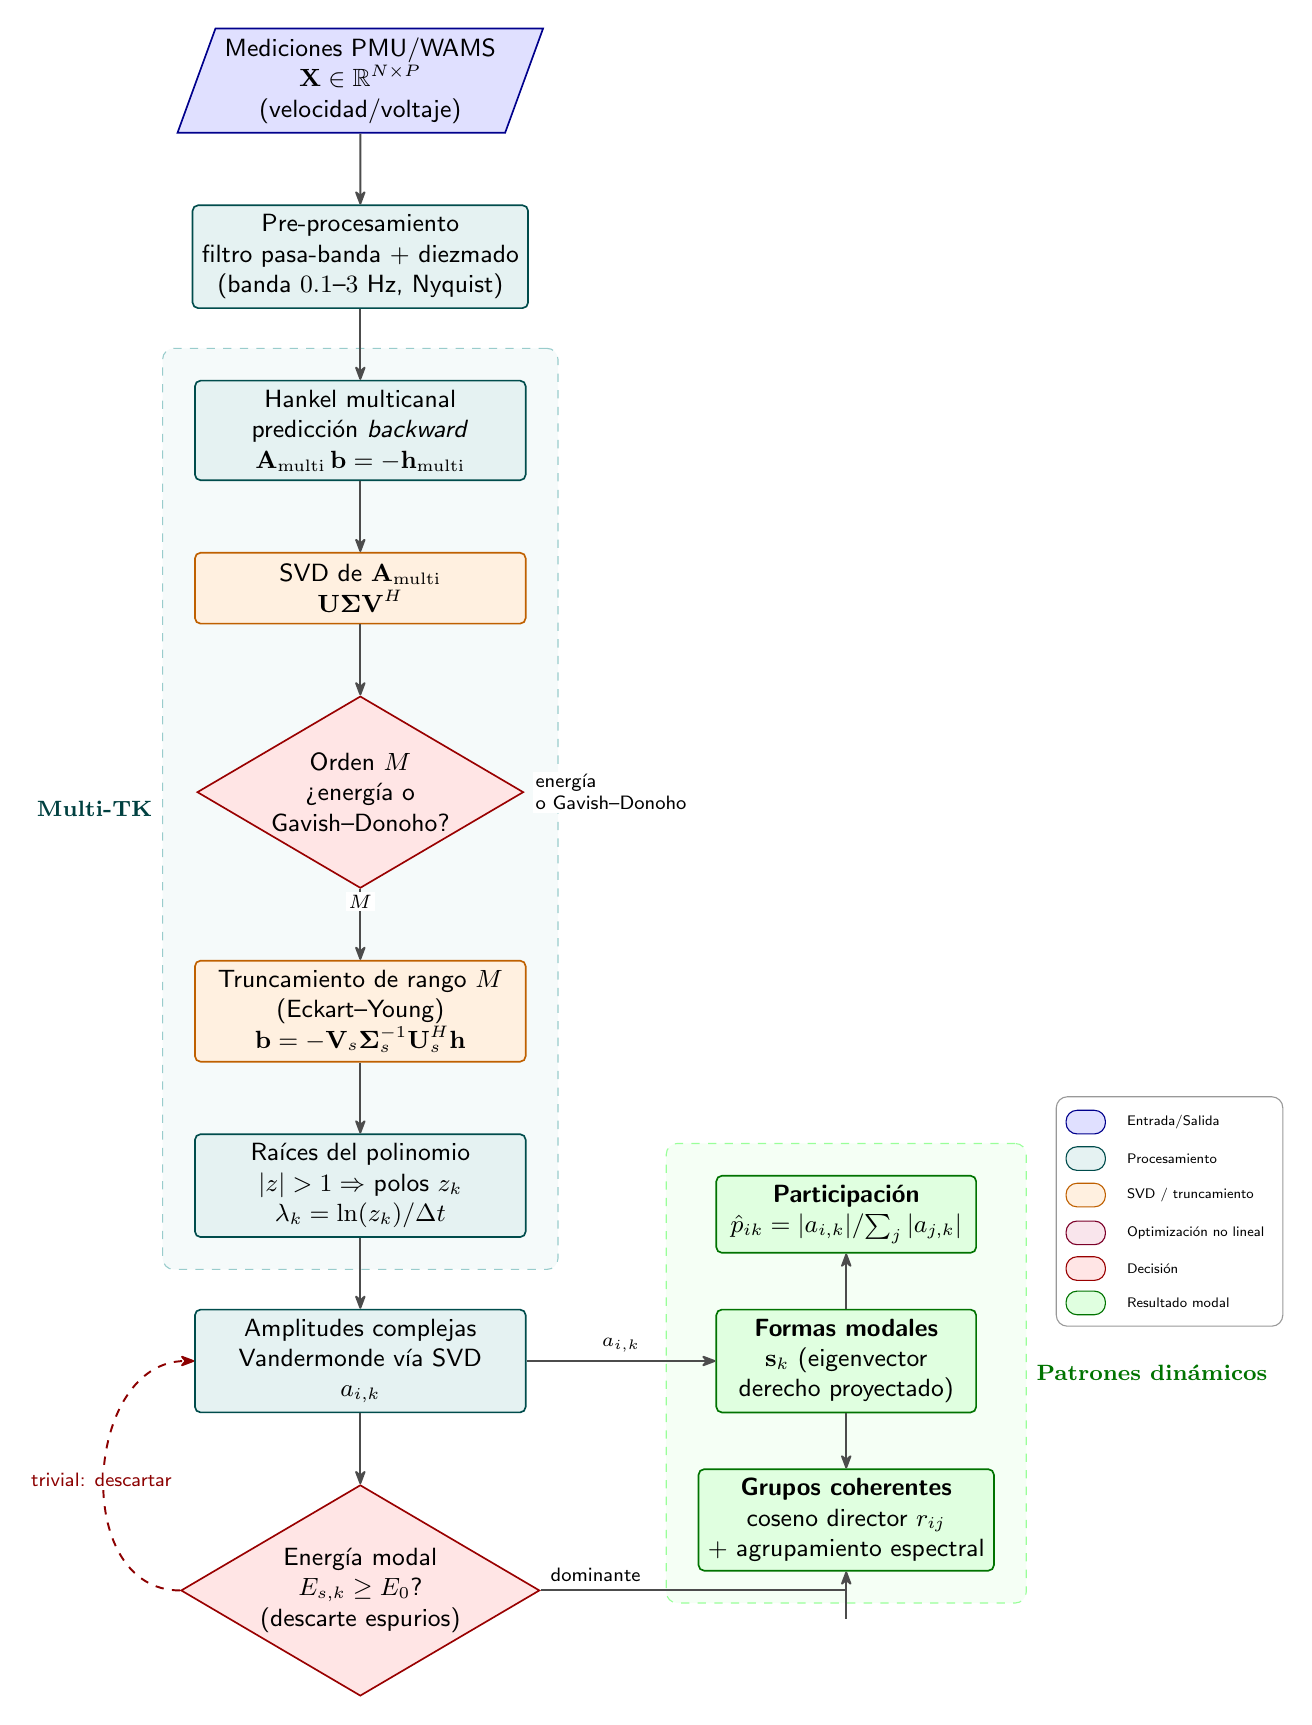
\begin{tikzpicture}[
    font=\small\sffamily,
    >={Stealth[round]},
    node distance = 9mm and 14mm,
    % --- estilos de caja ---
    io/.style    = {trapezium, trapezium left angle=70, trapezium right angle=110,
                    minimum width=30mm, minimum height=9mm, align=center,
                    draw=blue!55!black, fill=blue!12, line width=0.6pt},
    proc/.style  = {rectangle, rounded corners=2pt, minimum width=42mm,
                    minimum height=9mm, align=center,
                    draw=teal!60!black, fill=teal!10, line width=0.6pt},
    svd/.style   = {rectangle, rounded corners=2pt, minimum width=42mm,
                    minimum height=9mm, align=center,
                    draw=orange!75!black, fill=orange!12, line width=0.6pt},
    opt/.style   = {rectangle, rounded corners=2pt, minimum width=42mm,
                    minimum height=9mm, align=center,
                    draw=purple!65!black, fill=purple!10, line width=0.6pt},
    dec/.style   = {diamond, aspect=1.7, minimum width=30mm, align=center,
                    draw=red!60!black, fill=red!10, line width=0.6pt, inner sep=1pt},
    res/.style   = {rectangle, rounded corners=2pt, minimum width=33mm,
                    minimum height=9mm, align=center,
                    draw=green!45!black, fill=green!12, line width=0.6pt},
    arr/.style   = {->, line width=0.7pt, draw=black!70},
    lbl/.style   = {font=\scriptsize\sffamily, fill=white, inner sep=1pt}
]

% ===================== COLUMNA PRINCIPAL =====================
\node[io]   (data)  {Mediciones PMU/WAMS\\ $\mathbf{X}\in\mathbb{R}^{N\times P}$\\ (velocidad/voltaje)};
\node[proc] (pre)   [below=of data] {Pre-procesamiento\\ filtro pasa-banda $+$ diezmado\\ (banda $0.1$--$3$~Hz, Nyquist)};
\node[proc] (hank)  [below=of pre]  {Hankel multicanal\\ predicción \emph{backward}\\ $\mathbf{A}_{\mathrm{multi}}\,\mathbf{b}=-\mathbf{h}_{\mathrm{multi}}$};
\node[svd]  (svd)   [below=of hank] {SVD de $\mathbf{A}_{\mathrm{multi}}$\\ $\mathbf{U}\boldsymbol{\Sigma}\mathbf{V}^{H}$};
\node[dec]  (orden) [below=of svd]  {Orden $M$\\ ¿energía o\\ Gavish--Donoho?};
\node[svd]  (trunc) [below=of orden]{Truncamiento de rango $M$\\ (Eckart--Young)\\ $\mathbf{b}=-\mathbf{V}_s\boldsymbol{\Sigma}_s^{-1}\mathbf{U}_s^{H}\mathbf{h}$};
\node[proc] (roots) [below=of trunc]{Raíces del polinomio\\ $|z|>1 \Rightarrow$ polos $z_k$\\ $\lambda_k=\ln(z_k)/\Delta t$};
% --- Nodo OptVarPro ELIMINADO ---
\node[proc] (amp)   [below=of roots]{Amplitudes complejas\\ Vandermonde vía SVD\\ $a_{i,k}$};  % ahora debajo de roots
\node[dec]  (ener)  [below=of amp]  {Energía modal\\ $E_{s,k}\ge E_0$?\\ (descarte espurios)};

% ===================== RAMA DE PATRONES (derecha) =====================
\node[res] (shape) [right=24mm of amp]    {\textbf{Formas modales}\\ $\mathbf{s}_k$ (eigenvector\\ derecho proyectado)};
\node[res] (part)  [above=7mm of shape]   {\textbf{Participación}\\ $\hat p_{ik}=|a_{i,k}|/\!\sum_j|a_{j,k}|$};
\node[res] (coh)   [below=7mm of shape]   {\textbf{Grupos coherentes}\\ coseno director $r_{ij}$\\ $+$ agrupamiento espectral};

% ===================== FLECHAS PRINCIPALES =====================
\draw[arr] (data)  -- (pre);
\draw[arr] (pre)   -- (hank);
\draw[arr] (hank)  -- (svd);
\draw[arr] (svd)   -- (orden);
\draw[arr] (orden) -- (trunc);
\draw[arr] (trunc) -- (roots);
% Flecha directa de roots a amp (antes pasaba por varpro)
\draw[arr] (roots) -- (amp);
\draw[arr] (amp)   -- (ener);

% Etiqueta del orden M sobre la flecha orden->trunc
\node[lbl] at ($(orden)!0.5!(trunc)$) {$M$};

% Criterios de selección de orden
\node[lbl, right=1mm of orden, align=left] {energ\'ia\\ o Gavish--Donoho};

% Energía modal: si pasa (dominante) alimenta los patrones
\draw[arr] (ener.east) -| ($(coh.south)+(0,-6mm)$) -- (coh.south);
\node[lbl] at ($(ener.east)+(7mm,2mm)$) {dominante};

% Amplitudes -> formas modales
\draw[arr] (amp.east) -- (shape.west);
\node[lbl] at ($(amp.east)!0.5!(shape.west)+(0,2mm)$) {$a_{i,k}$};

\draw[arr] (shape.north) -- (part.south);
\draw[arr] (shape.south) -- (coh.north);

% Retro de descarte (modo trivial vuelve, lazo corto a la izquierda)
\draw[arr, dashed, draw=red!55!black]
    (ener.west) .. controls +(-1.4,0) and +(-1.4,0) .. (amp.west);
\node[lbl, text=red!55!black] at ($(ener.west)+(-1.0,1.4)$) {trivial: descartar};

% ===================== FONDOS POR ETAPA =====================
\begin{scope}[on background layer]
    \node[draw=teal!40, dashed, rounded corners, fill=teal!4, inner sep=4mm,
          fit=(hank)(roots), label={[teal!50!black,font=\footnotesize\bfseries]left:Multi-TK}] {};
    % --- CAJA OptVarPro ELIMINADA ---
    \node[draw=green!40, dashed, rounded corners, fill=green!4, inner sep=4mm,
          fit=(part)(shape)(coh),
          label={[green!45!black,font=\footnotesize\bfseries]right:Patrones dinámicos}] {};
\end{scope}

% ===================== LEYENDA =====================
\matrix [draw=black!40, rounded corners, fill=white, anchor=north west,
         column sep=1.5mm, row sep=0.8mm, font=\tiny\sffamily,
         every node/.style={anchor=west}]
    at ($(part.north east)+(10mm,10mm)$) {
    \node[draw=blue!55!black,   fill=blue!12,   minimum width=5mm, minimum height=3mm]{}; & \node{Entrada/Salida}; \\
    \node[draw=teal!60!black,   fill=teal!10,   minimum width=5mm, minimum height=3mm]{}; & \node{Procesamiento}; \\
    \node[draw=orange!75!black, fill=orange!12, minimum width=5mm, minimum height=3mm]{}; & \node{SVD / truncamiento}; \\
    \node[draw=purple!65!black, fill=purple!10, minimum width=5mm, minimum height=3mm]{}; & \node{Optimizaci\'on no lineal}; \\
    \node[draw=red!60!black,    fill=red!10,    minimum width=5mm, minimum height=3mm]{}; & \node{Decisi\'on}; \\
    \node[draw=green!45!black,  fill=green!12,  minimum width=5mm, minimum height=3mm]{}; & \node{Resultado modal}; \\
};

\end{tikzpicture}
\endgroup

% ---------- cierre del bloque standalone (descomentar si se activa arriba) ----------
\end{document}}
%     \caption[...]{...}
%     \label{fig:metodologia}
%   \end{figure}
%   NO compiles este archivo por separado (a menos que descomentes el bloque standalone).
%
% PAQUETES requeridos en el preámbulo de la tesis (¡imprescindibles!)

% ---------- BLOQUE STANDALONE (comentado; descomentar solo para prueba) ----------
 \documentclass[border=6pt]{standalone}
 \usepackage[utf8]{inputenc}
 \usepackage[T1]{fontenc}
 \usepackage{amsmath}
\usepackage{amssymb}
 \usepackage{tikz} \usetikzlibrary{shapes.geometric, arrows.meta, positioning, calc, fit, backgrounds}
 \begin{document}
% ------------------------------------------------------------------------

% Protección para babel español: desactiva localmente los shorthands < y >
% que interfieren con las puntas de flecha de TikZ (>={Stealth}, ->, -|).
\begingroup
\ifcsname shorthandoff\endcsname
  \shorthandoff{<>}
\fi
%
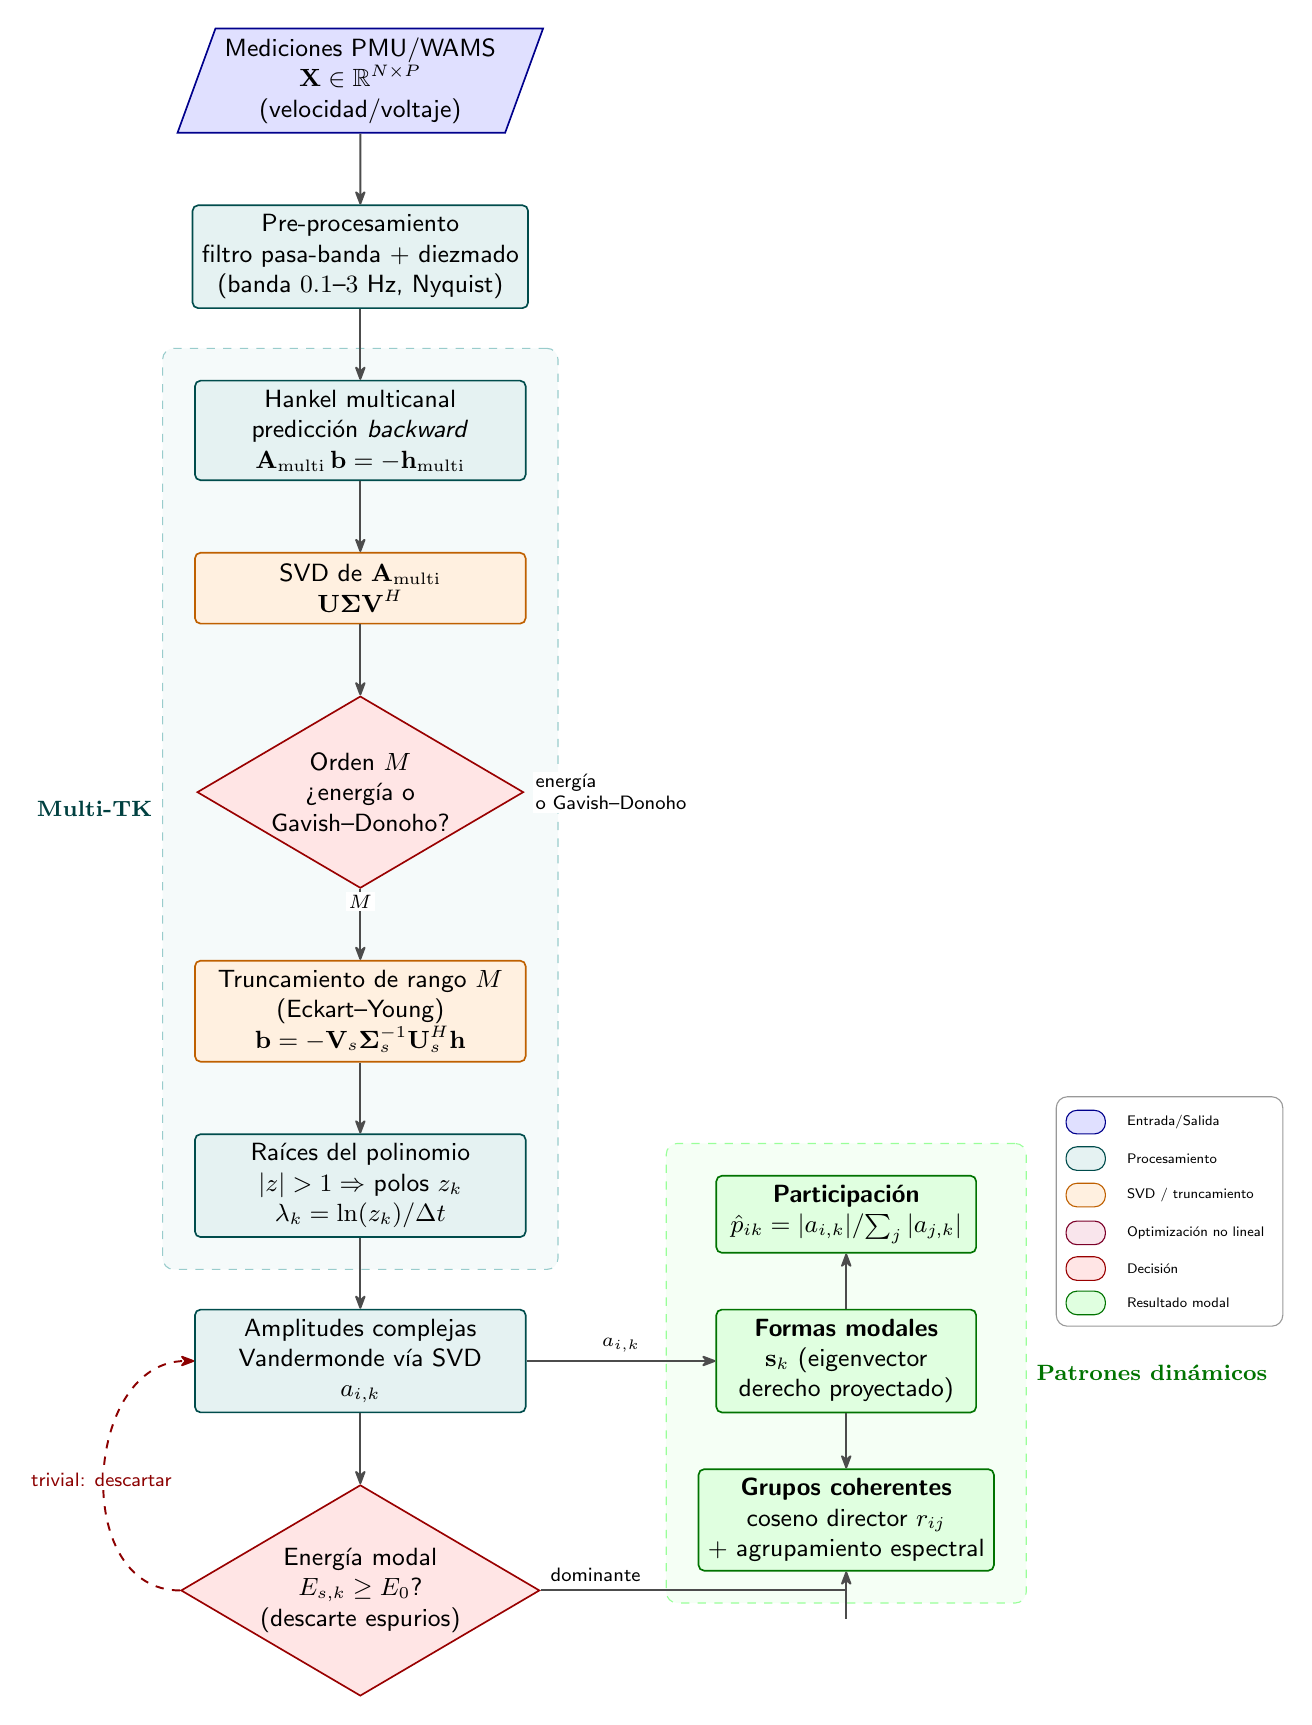
\begin{tikzpicture}[
    font=\small\sffamily,
    >={Stealth[round]},
    node distance = 9mm and 14mm,
    % --- estilos de caja ---
    io/.style    = {trapezium, trapezium left angle=70, trapezium right angle=110,
                    minimum width=30mm, minimum height=9mm, align=center,
                    draw=blue!55!black, fill=blue!12, line width=0.6pt},
    proc/.style  = {rectangle, rounded corners=2pt, minimum width=42mm,
                    minimum height=9mm, align=center,
                    draw=teal!60!black, fill=teal!10, line width=0.6pt},
    svd/.style   = {rectangle, rounded corners=2pt, minimum width=42mm,
                    minimum height=9mm, align=center,
                    draw=orange!75!black, fill=orange!12, line width=0.6pt},
    opt/.style   = {rectangle, rounded corners=2pt, minimum width=42mm,
                    minimum height=9mm, align=center,
                    draw=purple!65!black, fill=purple!10, line width=0.6pt},
    dec/.style   = {diamond, aspect=1.7, minimum width=30mm, align=center,
                    draw=red!60!black, fill=red!10, line width=0.6pt, inner sep=1pt},
    res/.style   = {rectangle, rounded corners=2pt, minimum width=33mm,
                    minimum height=9mm, align=center,
                    draw=green!45!black, fill=green!12, line width=0.6pt},
    arr/.style   = {->, line width=0.7pt, draw=black!70},
    lbl/.style   = {font=\scriptsize\sffamily, fill=white, inner sep=1pt}
]

% ===================== COLUMNA PRINCIPAL =====================
\node[io]   (data)  {Mediciones PMU/WAMS\\ $\mathbf{X}\in\mathbb{R}^{N\times P}$\\ (velocidad/voltaje)};
\node[proc] (pre)   [below=of data] {Pre-procesamiento\\ filtro pasa-banda $+$ diezmado\\ (banda $0.1$--$3$~Hz, Nyquist)};
\node[proc] (hank)  [below=of pre]  {Hankel multicanal\\ predicción \emph{backward}\\ $\mathbf{A}_{\mathrm{multi}}\,\mathbf{b}=-\mathbf{h}_{\mathrm{multi}}$};
\node[svd]  (svd)   [below=of hank] {SVD de $\mathbf{A}_{\mathrm{multi}}$\\ $\mathbf{U}\boldsymbol{\Sigma}\mathbf{V}^{H}$};
\node[dec]  (orden) [below=of svd]  {Orden $M$\\ ¿energía o\\ Gavish--Donoho?};
\node[svd]  (trunc) [below=of orden]{Truncamiento de rango $M$\\ (Eckart--Young)\\ $\mathbf{b}=-\mathbf{V}_s\boldsymbol{\Sigma}_s^{-1}\mathbf{U}_s^{H}\mathbf{h}$};
\node[proc] (roots) [below=of trunc]{Raíces del polinomio\\ $|z|>1 \Rightarrow$ polos $z_k$\\ $\lambda_k=\ln(z_k)/\Delta t$};
% --- Nodo OptVarPro ELIMINADO ---
\node[proc] (amp)   [below=of roots]{Amplitudes complejas\\ Vandermonde vía SVD\\ $a_{i,k}$};  % ahora debajo de roots
\node[dec]  (ener)  [below=of amp]  {Energía modal\\ $E_{s,k}\ge E_0$?\\ (descarte espurios)};

% ===================== RAMA DE PATRONES (derecha) =====================
\node[res] (shape) [right=24mm of amp]    {\textbf{Formas modales}\\ $\mathbf{s}_k$ (eigenvector\\ derecho proyectado)};
\node[res] (part)  [above=7mm of shape]   {\textbf{Participación}\\ $\hat p_{ik}=|a_{i,k}|/\!\sum_j|a_{j,k}|$};
\node[res] (coh)   [below=7mm of shape]   {\textbf{Grupos coherentes}\\ coseno director $r_{ij}$\\ $+$ agrupamiento espectral};

% ===================== FLECHAS PRINCIPALES =====================
\draw[arr] (data)  -- (pre);
\draw[arr] (pre)   -- (hank);
\draw[arr] (hank)  -- (svd);
\draw[arr] (svd)   -- (orden);
\draw[arr] (orden) -- (trunc);
\draw[arr] (trunc) -- (roots);
% Flecha directa de roots a amp (antes pasaba por varpro)
\draw[arr] (roots) -- (amp);
\draw[arr] (amp)   -- (ener);

% Etiqueta del orden M sobre la flecha orden->trunc
\node[lbl] at ($(orden)!0.5!(trunc)$) {$M$};

% Criterios de selección de orden
\node[lbl, right=1mm of orden, align=left] {energ\'ia\\ o Gavish--Donoho};

% Energía modal: si pasa (dominante) alimenta los patrones
\draw[arr] (ener.east) -| ($(coh.south)+(0,-6mm)$) -- (coh.south);
\node[lbl] at ($(ener.east)+(7mm,2mm)$) {dominante};

% Amplitudes -> formas modales
\draw[arr] (amp.east) -- (shape.west);
\node[lbl] at ($(amp.east)!0.5!(shape.west)+(0,2mm)$) {$a_{i,k}$};

\draw[arr] (shape.north) -- (part.south);
\draw[arr] (shape.south) -- (coh.north);

% Retro de descarte (modo trivial vuelve, lazo corto a la izquierda)
\draw[arr, dashed, draw=red!55!black]
    (ener.west) .. controls +(-1.4,0) and +(-1.4,0) .. (amp.west);
\node[lbl, text=red!55!black] at ($(ener.west)+(-1.0,1.4)$) {trivial: descartar};

% ===================== FONDOS POR ETAPA =====================
\begin{scope}[on background layer]
    \node[draw=teal!40, dashed, rounded corners, fill=teal!4, inner sep=4mm,
          fit=(hank)(roots), label={[teal!50!black,font=\footnotesize\bfseries]left:Multi-TK}] {};
    % --- CAJA OptVarPro ELIMINADA ---
    \node[draw=green!40, dashed, rounded corners, fill=green!4, inner sep=4mm,
          fit=(part)(shape)(coh),
          label={[green!45!black,font=\footnotesize\bfseries]right:Patrones dinámicos}] {};
\end{scope}

% ===================== LEYENDA =====================
\matrix [draw=black!40, rounded corners, fill=white, anchor=north west,
         column sep=1.5mm, row sep=0.8mm, font=\tiny\sffamily,
         every node/.style={anchor=west}]
    at ($(part.north east)+(10mm,10mm)$) {
    \node[draw=blue!55!black,   fill=blue!12,   minimum width=5mm, minimum height=3mm]{}; & \node{Entrada/Salida}; \\
    \node[draw=teal!60!black,   fill=teal!10,   minimum width=5mm, minimum height=3mm]{}; & \node{Procesamiento}; \\
    \node[draw=orange!75!black, fill=orange!12, minimum width=5mm, minimum height=3mm]{}; & \node{SVD / truncamiento}; \\
    \node[draw=purple!65!black, fill=purple!10, minimum width=5mm, minimum height=3mm]{}; & \node{Optimizaci\'on no lineal}; \\
    \node[draw=red!60!black,    fill=red!10,    minimum width=5mm, minimum height=3mm]{}; & \node{Decisi\'on}; \\
    \node[draw=green!45!black,  fill=green!12,  minimum width=5mm, minimum height=3mm]{}; & \node{Resultado modal}; \\
};

\end{tikzpicture}
\endgroup

% ---------- cierre del bloque standalone (descomentar si se activa arriba) ----------
\end{document}}
%     \caption[...]{...}
%     \label{fig:metodologia}
%   \end{figure}
%   NO compiles este archivo por separado (a menos que descomentes el bloque standalone).
%
% PAQUETES requeridos en el preámbulo de la tesis (¡imprescindibles!)

% ---------- BLOQUE STANDALONE (comentado; descomentar solo para prueba) ----------
 \documentclass[border=6pt]{standalone}
 \usepackage[utf8]{inputenc}
 \usepackage[T1]{fontenc}
 \usepackage{amsmath}
\usepackage{amssymb}
 \usepackage{tikz} \usetikzlibrary{shapes.geometric, arrows.meta, positioning, calc, fit, backgrounds}
 \begin{document}
% ------------------------------------------------------------------------

% Protección para babel español: desactiva localmente los shorthands < y >
% que interfieren con las puntas de flecha de TikZ (>={Stealth}, ->, -|).
\begingroup
\ifcsname shorthandoff\endcsname
  \shorthandoff{<>}
\fi
%
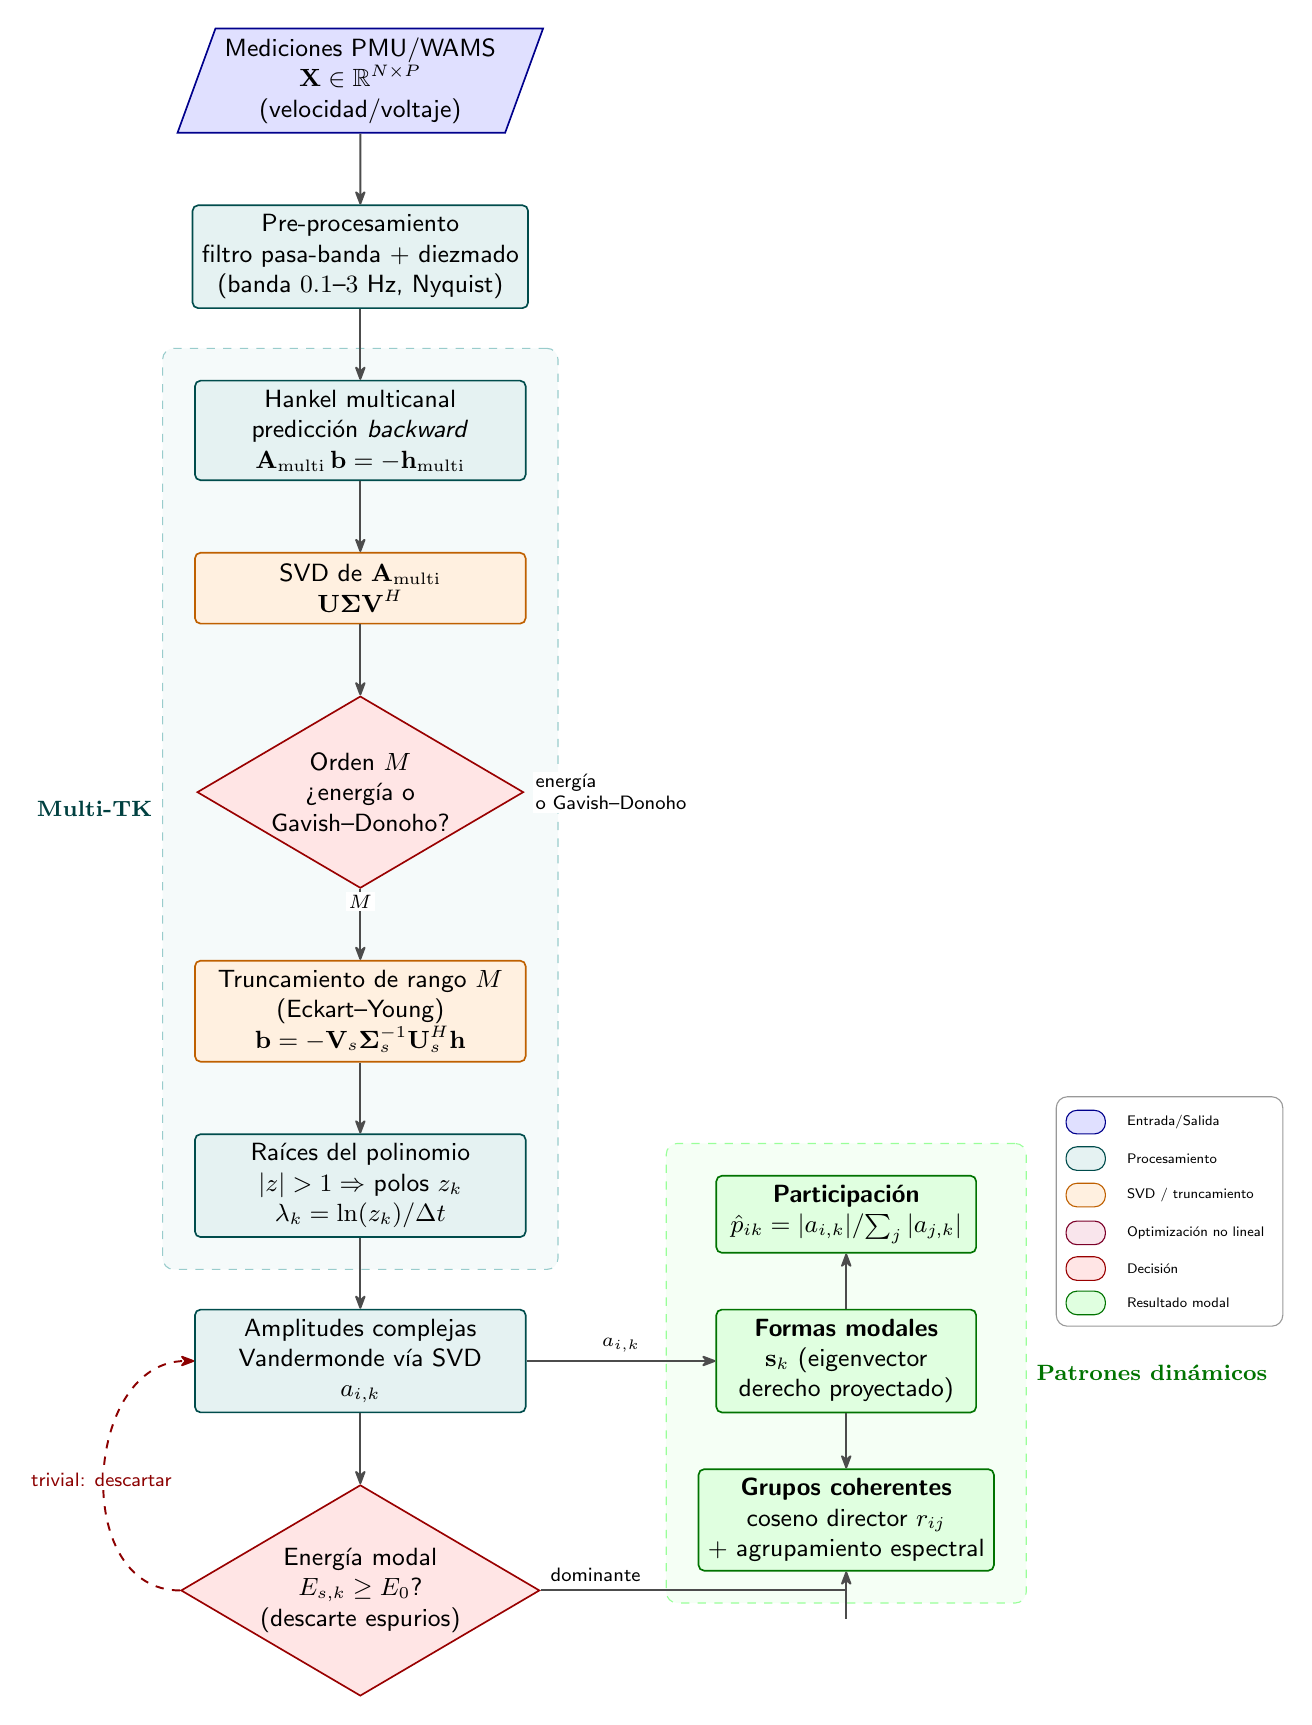
\begin{tikzpicture}[
    font=\small\sffamily,
    >={Stealth[round]},
    node distance = 9mm and 14mm,
    % --- estilos de caja ---
    io/.style    = {trapezium, trapezium left angle=70, trapezium right angle=110,
                    minimum width=30mm, minimum height=9mm, align=center,
                    draw=blue!55!black, fill=blue!12, line width=0.6pt},
    proc/.style  = {rectangle, rounded corners=2pt, minimum width=42mm,
                    minimum height=9mm, align=center,
                    draw=teal!60!black, fill=teal!10, line width=0.6pt},
    svd/.style   = {rectangle, rounded corners=2pt, minimum width=42mm,
                    minimum height=9mm, align=center,
                    draw=orange!75!black, fill=orange!12, line width=0.6pt},
    opt/.style   = {rectangle, rounded corners=2pt, minimum width=42mm,
                    minimum height=9mm, align=center,
                    draw=purple!65!black, fill=purple!10, line width=0.6pt},
    dec/.style   = {diamond, aspect=1.7, minimum width=30mm, align=center,
                    draw=red!60!black, fill=red!10, line width=0.6pt, inner sep=1pt},
    res/.style   = {rectangle, rounded corners=2pt, minimum width=33mm,
                    minimum height=9mm, align=center,
                    draw=green!45!black, fill=green!12, line width=0.6pt},
    arr/.style   = {->, line width=0.7pt, draw=black!70},
    lbl/.style   = {font=\scriptsize\sffamily, fill=white, inner sep=1pt}
]

% ===================== COLUMNA PRINCIPAL =====================
\node[io]   (data)  {Mediciones PMU/WAMS\\ $\mathbf{X}\in\mathbb{R}^{N\times P}$\\ (velocidad/voltaje)};
\node[proc] (pre)   [below=of data] {Pre-procesamiento\\ filtro pasa-banda $+$ diezmado\\ (banda $0.1$--$3$~Hz, Nyquist)};
\node[proc] (hank)  [below=of pre]  {Hankel multicanal\\ predicción \emph{backward}\\ $\mathbf{A}_{\mathrm{multi}}\,\mathbf{b}=-\mathbf{h}_{\mathrm{multi}}$};
\node[svd]  (svd)   [below=of hank] {SVD de $\mathbf{A}_{\mathrm{multi}}$\\ $\mathbf{U}\boldsymbol{\Sigma}\mathbf{V}^{H}$};
\node[dec]  (orden) [below=of svd]  {Orden $M$\\ ¿energía o\\ Gavish--Donoho?};
\node[svd]  (trunc) [below=of orden]{Truncamiento de rango $M$\\ (Eckart--Young)\\ $\mathbf{b}=-\mathbf{V}_s\boldsymbol{\Sigma}_s^{-1}\mathbf{U}_s^{H}\mathbf{h}$};
\node[proc] (roots) [below=of trunc]{Raíces del polinomio\\ $|z|>1 \Rightarrow$ polos $z_k$\\ $\lambda_k=\ln(z_k)/\Delta t$};
% --- Nodo OptVarPro ELIMINADO ---
\node[proc] (amp)   [below=of roots]{Amplitudes complejas\\ Vandermonde vía SVD\\ $a_{i,k}$};  % ahora debajo de roots
\node[dec]  (ener)  [below=of amp]  {Energía modal\\ $E_{s,k}\ge E_0$?\\ (descarte espurios)};

% ===================== RAMA DE PATRONES (derecha) =====================
\node[res] (shape) [right=24mm of amp]    {\textbf{Formas modales}\\ $\mathbf{s}_k$ (eigenvector\\ derecho proyectado)};
\node[res] (part)  [above=7mm of shape]   {\textbf{Participación}\\ $\hat p_{ik}=|a_{i,k}|/\!\sum_j|a_{j,k}|$};
\node[res] (coh)   [below=7mm of shape]   {\textbf{Grupos coherentes}\\ coseno director $r_{ij}$\\ $+$ agrupamiento espectral};

% ===================== FLECHAS PRINCIPALES =====================
\draw[arr] (data)  -- (pre);
\draw[arr] (pre)   -- (hank);
\draw[arr] (hank)  -- (svd);
\draw[arr] (svd)   -- (orden);
\draw[arr] (orden) -- (trunc);
\draw[arr] (trunc) -- (roots);
% Flecha directa de roots a amp (antes pasaba por varpro)
\draw[arr] (roots) -- (amp);
\draw[arr] (amp)   -- (ener);

% Etiqueta del orden M sobre la flecha orden->trunc
\node[lbl] at ($(orden)!0.5!(trunc)$) {$M$};

% Criterios de selección de orden
\node[lbl, right=1mm of orden, align=left] {energ\'ia\\ o Gavish--Donoho};

% Energía modal: si pasa (dominante) alimenta los patrones
\draw[arr] (ener.east) -| ($(coh.south)+(0,-6mm)$) -- (coh.south);
\node[lbl] at ($(ener.east)+(7mm,2mm)$) {dominante};

% Amplitudes -> formas modales
\draw[arr] (amp.east) -- (shape.west);
\node[lbl] at ($(amp.east)!0.5!(shape.west)+(0,2mm)$) {$a_{i,k}$};

\draw[arr] (shape.north) -- (part.south);
\draw[arr] (shape.south) -- (coh.north);

% Retro de descarte (modo trivial vuelve, lazo corto a la izquierda)
\draw[arr, dashed, draw=red!55!black]
    (ener.west) .. controls +(-1.4,0) and +(-1.4,0) .. (amp.west);
\node[lbl, text=red!55!black] at ($(ener.west)+(-1.0,1.4)$) {trivial: descartar};

% ===================== FONDOS POR ETAPA =====================
\begin{scope}[on background layer]
    \node[draw=teal!40, dashed, rounded corners, fill=teal!4, inner sep=4mm,
          fit=(hank)(roots), label={[teal!50!black,font=\footnotesize\bfseries]left:Multi-TK}] {};
    % --- CAJA OptVarPro ELIMINADA ---
    \node[draw=green!40, dashed, rounded corners, fill=green!4, inner sep=4mm,
          fit=(part)(shape)(coh),
          label={[green!45!black,font=\footnotesize\bfseries]right:Patrones dinámicos}] {};
\end{scope}

% ===================== LEYENDA =====================
\matrix [draw=black!40, rounded corners, fill=white, anchor=north west,
         column sep=1.5mm, row sep=0.8mm, font=\tiny\sffamily,
         every node/.style={anchor=west}]
    at ($(part.north east)+(10mm,10mm)$) {
    \node[draw=blue!55!black,   fill=blue!12,   minimum width=5mm, minimum height=3mm]{}; & \node{Entrada/Salida}; \\
    \node[draw=teal!60!black,   fill=teal!10,   minimum width=5mm, minimum height=3mm]{}; & \node{Procesamiento}; \\
    \node[draw=orange!75!black, fill=orange!12, minimum width=5mm, minimum height=3mm]{}; & \node{SVD / truncamiento}; \\
    \node[draw=purple!65!black, fill=purple!10, minimum width=5mm, minimum height=3mm]{}; & \node{Optimizaci\'on no lineal}; \\
    \node[draw=red!60!black,    fill=red!10,    minimum width=5mm, minimum height=3mm]{}; & \node{Decisi\'on}; \\
    \node[draw=green!45!black,  fill=green!12,  minimum width=5mm, minimum height=3mm]{}; & \node{Resultado modal}; \\
};

\end{tikzpicture}
\endgroup

% ---------- cierre del bloque standalone (descomentar si se activa arriba) ----------
\end{document}
     \caption{Diagrama de flujo de la metodología}
     \label{fig:metodologia}
 \end{figure}

\chapterbibliography%